% Tento soubor nahraďte vlastním souborem s obsahem práce.
%=========================================================================
% Autoři: Michal Bidlo, Bohuslav Křena, Jaroslav Dytrych, Petr Veigend a Adam Herout 2019
\chapter{Úvod}
Zde bude cca jedna strana úvod…

\blindtext[2]
\todo{Upravit}.


\chapter{Automatizace domácnosti}
Následující část je shrnutím současného stavu v oblasti automatizace domácnosti a chytrých domovů. Není encyklopedickým výkladem problematiky, ale souhrnem informací, které mají k práci bezprostřední vztah. Nejprve je zde popis automatizace domácnosti, co to je, jaké jsou dnes možnosti jejího využití, přínosy a používané principy.

\section{Automatizace domácnosti a chytrý dům}
Automatizace domácnosti spočívá v automatizování činností, které řídí domácnost, normálně vykonávané člověkem. Můžeme ji definovat jako mechanismus, který nahrazuje lidskou námahu (při ovládání domácnosti), natolik, nakolik je to jen možné [U]. V souvislosti s tím někdy hovoříme o inteligentní, řízené či chytré domácnosti. Jedná se o kolekci zařízení a (pod)systémů, které jsou schopny spolu komunikovat či fungovat nezávisle. Přitom automatizovaný „dům budoucnosti“ slibují výrobci domácích zařízení prakticky již téměř od počátku minulého století [1]. Chytrý dům (či smart home) je pak definován jako dům, vybavený výpočetní a informační technologií, které předvídá uživatelovi potřeby a odpovídá na ně, a přitom dbá na jeho pohodlí, bezpečnost a zábavu [13]. Často se tedy tyto dva pojmy (automatizovaný a chytrý dům) zaměňují, ačkoli \todo{Z nějakého nového zdroje rozvést, viz odkaz}
\begin{verbatim}
https://www.google.com/search?q=smart+home+vs+home+automation&rlz=1C1AVFC_enCZ780CZ780&oq=smart+home+vs+hom&aqs=chrome.0.0i19j69i57j0i19i22i30j0i5i13i19i30l5.7375j0j7&sourceid=chrome&ie=UTF-8
\end{verbatim}




\subsection*{Možnosti využití automatizace v domácnosti}
Automatizace v mnohém usnadňuje život a umožňuje provádění akcí, které by jinak byli prakticky nemožné (například zabezpečení domu, efektivní řízení vytápění domácnosti a spotřeby energie). V současné době patří automatizace domácnosti mezi rychle se rozvíjející technologie \todo{Dopsat zdroj, viz  odkaz} []. 
\begin{verbatim}
https://www.google.com/search?q=home+automation+is+fast+developing&rlz=1C1AVFC_enCZ780CZ780&oq=home+automation+is+fast+deveopin&aqs=chrome.1.69i57j33i10i160.14343j0j7&sourceid=chrome&ie=UTF-8
\end{verbatim} 
Mezi typické aplikace automatizace domácnosti patří například:
\begin{itemize}
\item Zabezpečovací systém
\item Systém pro inteligentní vytápění a ventilaci (HVAC)
\item Zábava a multimédia
\item Komunikace
\item Osvětlení [3]
\item Ovládání spotřebičů [T]
\item Samo zavlažovací systémy [U]
\item A mnoho dalšího
\end{itemize}

\begin{figure}[hbt]
	\centering
	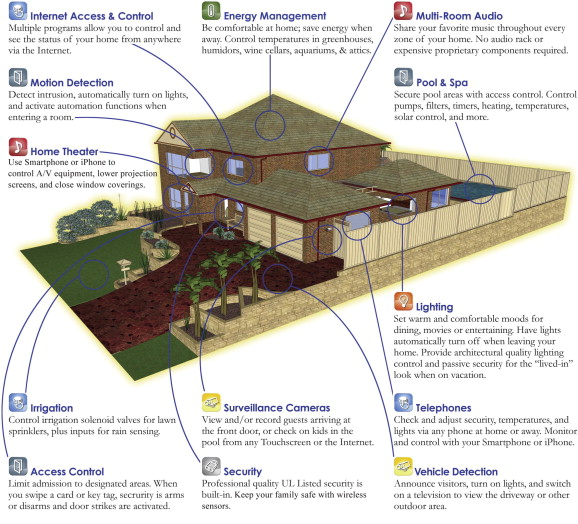
\includegraphics{obrazky/automation-example.jpg}
	\caption{Příklad možností automatizované domácnosti[U]}
	\label{asd}
\end{figure}
Nejaky text, mozna spise az sem o tom, že "V současné době patří automatizace domácnosti mezi rychle se rozvíjející technologie".


\newpage
\subsection*{Přínosy automatizace domácnosti}
Přidání inteligence do domácnosti přináší do života lidí řadu přínosů. Jde zejména o:

\begin{itemize}
\item Bezpečí – Chytré domy mohou používat různé senzory, které detekují nebezpečí a v souvislostí s nimi provést patřičné akce k jejich zabránění, případně minimalizaci škod. Příkladem mohou být záplavové a kouřové senzory a v neposlední řadě také zabezpečovací systém domácnosti.
\item Komfort – Chytré domácnosti svými funkcemi nabízejí různé způsoby, jak jejich uživatelům zpříjemnit různé rutinní akce. Mohou se postarat o automatické nastavování žaluzií dle intenzity venkovního světla, přes dotykový displej na dálku ztlumit světlo či hlasovým pokynem uvést celý byt do jiného světelného režimu. 
\item Přehled o provozu – Systémy pro automatizaci domácnosti zahrnují i displeje s přehledem o stavu jednotlivých zařízení a čidel. Také je v některých systémech možné tyto informace sledovat i z chytrých telefonů, tabletů či počítačů (a to i vzdáleně). V některých komplexnějších systémech, které například zahrnují komunikaci přes mobilní sítě je možné získávat přehled o provozu dokonce pomocí SMS zprávy (hodí se třeba při absenci internetového připojení) [15]
\item Úspora – V chytrých domácnostech je možné použít inteligentní vytápění domu založené na údajích z teplotních čidel, denní doby, případně nastaveném režimu domácnosti. Společnost ELKO EP odhaduje, že díky bezdrátové regulaci topení je možné ušetřit až 30 \% nákladů na energii [17]. Úsporu rovněž zajistí automatizovaná světla, o kterých je možné mít v automatizované domácnosti vždy přehled, na dálku je zapínat/vypínat dle potřeby a rovněž je napojit na senzory, které je budou ovládat například na základě přítomnosti osob v místnosti.
\end{itemize}
    

\subsection*{Základní klasifikace chytré domácnosti}
Chytrou domácnost můžeme rozdělit dle kabeláže:

\begin{itemize}
\item Drátovou
\item Bezdrátovou 
\item Kombinovanou
\end{itemize}
Pokud má být domácnost komplexně automatizovaná, je často vhodnější mít celý systém propojený pomocí kabelů, jelikož takový systém bude spolehlivější a v případě potřeby nabízí rychlejší přenos dat (například pokud mají být součástí systému multimédia). Bezdrátové systémy se hodí zejména tam, kde není žádané zasahovat do elektroinstalace, či pokud uživatel potřebuje pouze jednodušší systém (například s ovládáním několika málo zařízení). Připravená kabeláž pro automatizaci domácnosti rovněž přináší výhodu snadnějšího řešení napájení jednotlivých chytrých zařízení, které se tak může rozvádět po bytě spolu s datovými kabely. Přitom pro propojení jednotlivých chytrých zařízení mezi sebou je možné využít různé typy kabelů (např. ethernetový) [15]. Systémy s kombinovanou kabeláží pak vycházejí z klasické kabelové instalace s možností použití některých bezdrátových prvků (např. snímačů).


\subsection*{Mechanismy používané v chytrých domovech}
V chytrém domě se při automatizaci obvykle používají následující principy:

\begin{itemize}
\item Přímé ovládání spotřebičů
\item Nastavení scény
\item Podmínky [16, pokud neseženu lepší]
\end{itemize}
Přímé ovládání spotřebičů se obvykle provádí dálkovým ovládáním, používá-li spotřebič pro komunikaci technologii rádiového přenosu na frekvencích 443 MHz. Příkladem takového zařízení může být „bla bla bla“ od společnosti...Jiný způsob ovládání rovněž zahrnuje použití jiného chytrého zařízení (například chytrého telefonu), pokud ovládané zařízení umí komunikovat pomocí stejné technologie (např. WiFi). Ovládání pomocí telefonu či podobného chytrého zařízení je možné i v případě, že ovládané zařízení neumí komunikovat stejnou technologií, ale v domácnosti existuje centrální prvek (hub), který podporuje obě technologie a funguje zde jako prostředník mezi oběma zařízeními. \newline
V chytrých domovech je rovněž často možné použít rovněž nastavení některé předem definované scény. Tato scéna sdružuje několik příkazů přímého ovládání. Může se například jednat o scénu odchodu z domu, která vypne všechna světla, odpojí spotřebiče od elektrické sítě a aktivuje zabezpečovací systém.\newline
Dalším principem uplatňovaným v chytrém domě jsou nastavené podmínky. Ty způsobí, že při určité akci systém zareaguje nějakým předem nastaveným způsobem. Například se může jednat o podmínku, aby v případě že s….\newline

\subsection*{Komponenty chytré domácnosti}
Na trhu dnes existuje nepřeberné množství různých systémů. Typická automatizovaná domácnost využívá některé (či všechny) z následujících komponent: \newline

\begin{itemize}
\item Vstupní prvky (různá čidla, tlačítka, dotykové displeje…)
\item Výstupní prvky (Světla, spotřebiče a různá zařízení)
\item Virtuální (hlasový) asistent
\item Centrální jednotka
\item Aplikace pro řízení domácnosti z chytrých zařízení (telefonu, tabletu, počítače…)
\end{itemize}

\subsection*{Chytrá zařízení a IoT}
\todo{todo}

\subsection*{Protokoly používané v automatizaci domácnosti}
\todo{todo - MQTT atd...}
\todo{Možná změnit uplně kapitolu technol. bezdrátového přenosu na Protokoly a tam radši dát MQTT atd?}


\section{Virtuální hlasoví asistenti a centrální prvky chytré domácnosti}
Virtuální osobní asistent (VPA) je osobní asistent, který zajišťuje interakci mezi uživatelem chytré domácnosti a zařízeními v ní. Jako jiné označení se rovněž používá inteligentní či digitální osobní asistent, či mobilní asistent. Je-li ovládaný hlasem, pak se někdy označuje jako hlasový asistent [6]. Dále v textu této kapitoly je vždy asistentem míněn právě hlasový asistent, nebude-li specifikováno jinak. Jedná se o software, jehož úlohou je asistovat uživateli při nejrůznějších příležitostech, mezi jinými i při ovládání domácnosti. Hlasoví asistenti běží na některém zařízení s reproduktorem a mikrofony nebo mobilním zařízení. Dnes jich existuje na trhu veliké množství (zejména pro chytré telefony), mezi jejich nejznámější představitele v současné době patří:
\begin{itemize}
\item Apple Siri
\item Amazon Alexa
\item Microsoft Cortana
\item Google Assistant [2]
\item Samsung S voice
\item Facebook M
\item Nuance dragon [6]
\end{itemize}
V současné době žádný z výše uvedených hlasových systémů nepodporuje češtinu, nicméně Assistant od společnosti Google by ji v dohledné době mohl podporovat [14]. Amazon Alexa pak sice nerozumí česky, ale již dokáže číst některé knihy v češtině []ttt. Pro českého uživatele jsou tak pouze 2 možnosti – buďto používat asistenta v angličtině a spokojit se s případnou absencí některých funkcí, které nejsou v česku podporované (UVÉST KTERÉ A CITOVAT ZDROJ – NAPŘÍKLAD VOLÁNÍ JEN V USA, BEZTAK I NAKUPOVÁNÍ???), nebo použít některého českého virtuálního asistenta, ovšem s omezenou funkcionalitou oproti jejich „něco“ protějškům. Mezi české hlasové asistenty patří například:
\begin{itemize}
\item Emma
\item Intelli
\end{itemize}
Zmínit se o českých asistentech (EMMA, INTELLI) a najít další
\ subsection*{Použití virtuálních asistentů}
Každý z virtuálních asistentů má své vlastní specifikace, ovšem jsou typy úloh, které vykonávají více méně všichni asistenti:
\begin{itemize}
\item Číst a psát SMS a emailové zprávy, uskutečňovat hovory
\item Nastavovat časové a kalendářové akce (časovače, upomínky…)
\item Odpovídat na některé základní informativní otázky (počasí, čas, převody jednotek…)
\item Ovládat média jako televizi či připojené reproduktory (pouštět filmy, hudbu)
\item Vyprávět vtipy a příběhy
\item Konečně ovládat prvky chytré domácnosti [2]
\end{itemize}
Používání virtuálních osobních asistentů nejen, že umožňuje přistupovat k různým úkolům inovativním a interaktivním způsobem, ale v mnoha případech i zjednodušuje jinak relativně zdlouhavou činnost. Dobrým příkladem je například manuální nastavení budíku (bez použití VPA). Na mobilním telefonu (Nexus 5) je potřeba vykonat následující akce:
\begin{enumerate}
\item Kliknout na tlačítko pro návrat na domovskou obrazovku (pokud se tam uživatel nenachází)
\item Kliknout na ikonu hodin
\item V otevřené aplikaci najít ikonu budíku a kliknout na ni 
\item Kliknout na tlačítko „+“ pro přidání budíku
\item Nastavit hodinu, překliknout na volbu minuty a nastavit minuty
\item Potvrdit kliknutím na tlačítko „OK“
\end{enumerate}
Při použití hlasového asistenta je celá úloha značně zredukována pouze na aktivování asistenta a vyslovení požadovaného úkolu [6]. \newline
Bez použití VPA je dokonce řada úkolů nerealizovatelná. Například připomenout či udělat něco v okamžiku, kdy se uživatel vrátí domů, což je funkce, kterou někteří virtuální asistenti podporují [16]. Interaktivitu zajišťují virtuální asistenti i při automatizaci domácnosti, pro její řízení není potřeba otevírat k tomu určené (a mnohdy jednoúčelové) aplikace, ale stačí vyslovit žádost, třeba i s jistou vzdáleností od zařízení s hlasovým asistentem a ten se již o vše postará [DOLOŽIT!!!]. Kromě toho, virtuální asistenti v sobě mohou nést i funkce sloužící přímo pro automatizaci domácnosti. Například nastavení podmínek, scénářů atd [Rozveď to a uved nejaky zdroj!!!]. \newline
Virtuální asistenti díky svým funkcím a vlastnostem k chytré domácnosti neodmyslitelně patří, ovšem je nutné si uvědomit, že zde nejsou nutností. Spíše často fungují jako prostředník mezi uživatelem a chytrými zařízeními, který usnadňuje řízení domácnosti. Často pak bývají zabudováni do chytrého zařízení, plnící funkci centrálního prvku (hubu), jako například v případě zařízení Echo od společnosti Amazon. [DOLOŽIT NĚJAK!!!] \newline
\ subsection*{Amazon}
\ subsection*{Google}
\ subsection*{Microsoft}
\ subsection*{Apple}
\ subsection*{Emma}

Emma je český hlasový asistent, kterého vytvořil David Beck pomocí aplikace Zkratky (na systému iOS). Jak již bylo zmíněno, nativním virtuálním asistentem pro iPhone je Siry, ta však neumí česky, a to se rozhodl David Beck změnit [20]. Nejedná se o samostatnou aplikaci, ale o zkratku v aplikaci Zkratky na systému iOS. Tato aplikace zkratky umožňuje uživatelům sloučit různé akce do jedné zkratky. Celkově pro zkratku Emma nastavil 7 tisíc akcí a další se chystá přidávat. Systém v současné době již podporuje češtinu, částečně slovenštinu a polštinu. Plánuje také přidat maďarštinu, řečtinu a rumunštinu [21]. 

\section{Existující řešení chytrých domů}
Dnes je na trhu nepřeberné množství systémů, lišících se v ceně, komplexnosti, způsobem komunikace a podobně. Jednou z nejčastějších aplikací automatizace, kterou různé společnosti nabízejí je ovládání světel a zásuvek. Mezi další aplikace patří ovládání hlavic radiátorů, chytré termostaty, ovládání ventilátorů, stínící techniky, alarm a podobně. Mezi konkrétní systémy, které jsou dostupné na českém trhu patří:
\begin{itemize}
\item Loxone
\item Jablotron
\item Apple HomeKit
\item Sonoff
\item Fibaro
\item Homeconnect
\item A mnoho dalších
\end{itemize}
Kromě komerčně prodávaných systémů je k dispozici rovněž open source řešení, mezi známější patří například:
\begin{itemize}
\item Home Assistant
\item A další
\end{itemize}

\subsection*{Loxone}
Loxone je společnost, zaměřující se na automatizaci budov, v rozsahu od malých bytů, přes hotely až po rozsáhlé budovy a výrobní haly. Zaměřují se na širokou škálu aplikací, v oblasti automatizace domácnosti jde zejména o:
\begin{itemize}
\item Bezpečnost (Pohybové senzory, dveřní a okenní senzory)
\item Přístup do budovy (Přístup kódem zadávaným na klávesnici, NFC přívěškem či iButtonem, kamera)
\item Řízení filtrace bazénu
\item Větrání (Automatické řízení ventilace, například na základě přítomnosti osoby, vlhkosti, teplotě…)
\item Regulace teploty (Loxone je možné připojit k jakémukoli zdroji teploty i chlazení)
\item Úspora energie (Ovládání budovy k úsporám energie – například automatické stínění jako ochrana přetopení ze slunečního tepla)
\item Osvětlení (ovládání bodového světla, LED pásků či Loxone závěsných světel)
\item Multimédia (Ovládání audia, TV…)
\item Stínění (Ovládání stínící techniky pomáhá při vytápění a chlazení v domě)
\item A díky rozšířením také mnoho dalšího [32]
\end{itemize}
Systém loxone se skládá z několika různých prvků:

\begin{itemize}
\item Miniserver
\item Rozšíření
\item Příslušenství (Loxone Tree zařízení)
\item Loxone Tree a Loxone Link kabeláž
\item Aplikace Loxone App a Loxone Config
\end{itemize}
Loxone prvky ke své činnosti potřebují tzv. miniserver. Ten v systému funguje jako centrální řídící jednotka, která se stará o automatizaci domácnosti. Loxone nabízí celkem 3 různé verze miniserveru:

\begin{itemize}
\item Miniserver Gen. 1
\item Miniserver Gen. 2
\item Miniserver Go
\end{itemize}

Miniserver 1. i 2. generace mají oba 8 digitálních a 4 analogové vstupy a 8 digitálních výstupů (relé spínající max 250VAC/30VDC). Miniserver 1. generace má ještě navíc 4 analogové výstupy [27]. Obě generace miniserveru slouží pro kabelovou komunikaci a jsou určené k instalaci na DIN lištu. Také jsou obě generace vybaveny rozhraním Loxone Link (pro kabelové připojení až 30 tzv. rozšíření) a LAN port (Fast ethernet). Pouze první generace obsahuje KNX rozhraní, naopak pouze druhá generace a verze Go obsahují již integrované rozhraní Loxone Tree (K první generaci je pro komunikaci po Loxone Tree sběrnici dodat rozšiřující modul) [28]. \newline
Pokud si uživatel přeje využívat bezdrátové komunikace mezi prvky systému Loxone (zejména Pro bezdrátové ovládání pak Loxone nabízí 3. verzi miniserveru – Miniserver Go. Ten komunikuje s bezdrátovými periferiemi (rozšířeními a příslušenstvím) rádiovou komunikací na frekvenci 868MHz pro SRD pásmo pro Evropu (na 4 kanálech), případně 915MHz pro ITU region 2 (10 kanálů), s maximálním výkonem 3.16 mW [26]. Obsahuje také LAN port (Fast ethernet) a rozhraní Loxone Link. K této verzi miniserveru je možné bezdrátově připojit až 128 periferií [31].

\begin{figure}[hbt]
	\centering
	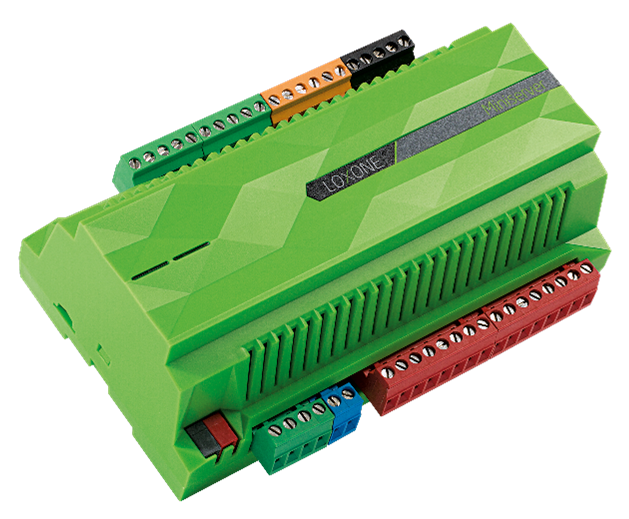
\includegraphics{obrazky/loxone-miniserver.png}
	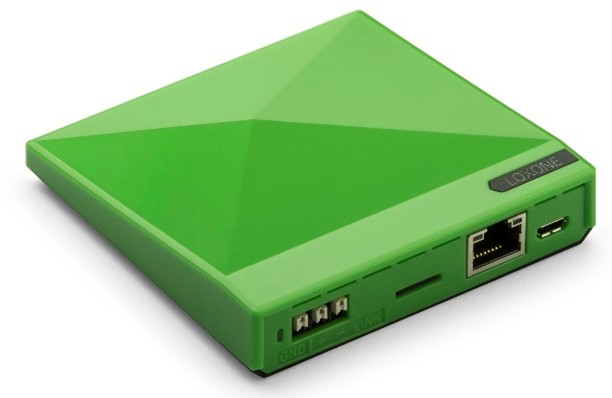
\includegraphics{obrazky/loxone-miniserver-go.jpg}
	\caption{Loxone Miniserver gen. 1 a Miniserver Go. Převzato z Loxone web}
	\label{miniserver}
\end{figure}


Všechny verze Miniserveru v sobě obsahují Loxone OS s integrovaný webový server, jsou konfigurovatelné z programu Loxone Config a ovladatelné přes mobilní aplikaci (Loxone App) [33]. Všechny miniservery obsahují slot pro SD kartu (s firmwarem). 

\begin{figure}[hbt]
	\centering
	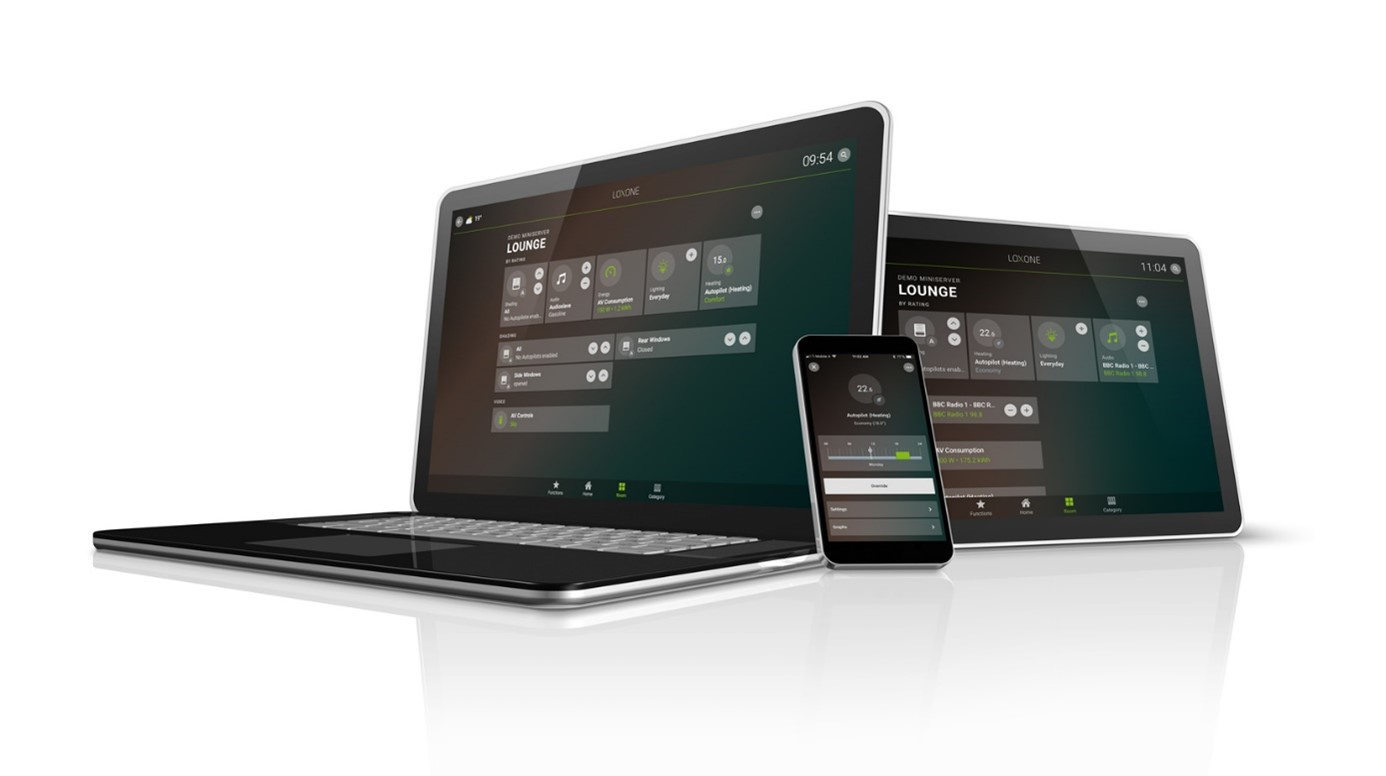
\includegraphics{obrazky/loxone-app.jpg}
	\caption{Loxone App. Převzato z Loxone web}
	\label{loxone-app}
\end{figure}

Loxone Extensions (rozšíření) slouží pro rozšíření funkcí Miniserveru. K Miniserveru se připojují pomocí sběrnice Loxone Link (kterou obsahují všechny verze Miniserveru). Tato sběrnice může být až 500 m dlouhá. Díky rozšířením může uživatel zakoupit systém pouze s těmi technologiemi, které chce opravdu využívat a nemusí tak platit za zbytečné vlastnosti systému. Příkladem rozšíření mohou být Tree Extension (pro připojení až 100 Tree zařízení; zejména pro doplnění Miniserveru 1. generace, který neobsahuje rozhraní pro komunikaci přes tree sběrnici) [36], Air Base Extension (Pro doplnění Miniserverů 1. a 2. gen – k bezdrátové komunikaci) [37], Dimmer Extension (pro stmívání světel) [38] a mnoho dalších.\newline
Loxone nabízí pro automatizaci domácnosti více než 400 produktů [33].
Loxone pro propojení prvků v systému vyvinulo tzv. Loxone Tree technologii. Jedná se o sběrnici, na kterou je možné připojit až 50 prvků, a Loxone uvádí, že díky tomu je možné ušetřit až 80\% kabeláže [DOLOŽIT!]. Podobně jako Loxone Link, i Loxone Tree může sahat až 500 m daleko. \newline

V oblasti inteligentního vytápění nabízí Loxone souhru technologií pro vytápění, chlazení, rekuperaci, a automatizovanou stínící techniku, což přináší do regulace vytápění vysokou efektivitu [34]. \newline
Z hlediska regulace teploty nabízí tzv. „zónové“ vytápění. Jedná se o inteligentní topení, které na rozdíl od klasického inteligentního vytápění (zahrnující obvykle nějaký bezdrátový termostat, wifi termostatické hlavice apod.) umožňuje inteligentněji řídit teplotu – tím že uživatel zvolí, ve které místnosti (případně i ve který čas) má být jaká teplota. Uživatel chytrého domu s tímto systémem si tak může navolit například větší teplo v koupelně oproti například místnosti kde spí. Tento systém tak umožňuje mít větší kontrolu nad vytápěnými místnostmi, potažmo vyšší efektivitu. \newline
Inteligentní vytápění Loxone podporuje režim učení, systém se tedy na základě předchozích zkušeností spustí vytápění tak, aby byla v dané místnosti požadovaná teplota ve správný čas. Uživatel si tak může nastavit například to, aby měl v 7:00 vyhřátou koupelnu na 23 °C. \newline
Loxone vytápění má dle oficiálních stránek [25] následující výhodné vlastnosti:
\begin{itemize}
    \item Inteligentní řízení teploty – využití již zmíněného režimu učení k dosažení požadované teploty v žádaný čas. Loxone rovněž při regulaci zohledňuje venkovní teplotu.
    \item Úspora nákladů – Loxone dokáže inteligentně rozhodovat o nejefektivnějším řešení. Například energeticky náročnou klimatizaci může nahradit energeticky výhodnějším stínění
    \item Režim nepřítomnosti – Systém od loxone podporuje úsporný režim pro chvíle, kdy uživatel není doma
    \item Ochrana budovy – Loxone dokáže reagovat na různá nebezpečí, například v případně vzniku požáru vypnout ventilaci i rekuperaci
    \item Loxone aplikace a statistiky – Loxone nabízí zdarma aplikaci na zařízení s androidem přes které uživatel může sledovat i nastavovat teplotu v domě vzdáleně
    \item Notifikace – V případě problému s některou technologií Loxone upozorní uživatele
    \item Státní svátky – Na základě znalosti státních svátků může Loxone adekvátně upravovat svoji činnost
    \item Údržba – Loxone uživatele upozorňuje na termín pravidelné údržby
\end{itemize}
Z hlediska automatizace domácnosti v porovnání s dříve uvedenými systémy je rovněž důležitá přítomnost ovládané chytré zásuvky. Ta s Miniserverem komunikuje technologií Loxone Air. Má v sobě teplotní čidlo a rovněž elektroměr s vyhodnocením výkonu a spotřeby \newline
//ještě zmínit loxone touch a tlačítko na stul \newline

\subsection*{Jablotron}
Jablotron je česká firma, která se od svého založení zaměřuje především na zabezpečovací systémy [40]. Kromě nich se také zabývá zabezpečením a monitoringem vozidel, topením a ventilací, monitoringem dechu a rovněž ovládáním a automatizací domácnosti [39]. \newline
Jablotron nabízí několik různých systémů. Dva nejnovější jsou Jablotron 100 a Jablotron 100+ [40]. Primárním úkolem obou systémů je zabezpečení budov, ovšem je možné je využít i v oblasti automatizace (zejména díky programovatelným výstupům). Samotné zabezpečení je možné využít v rámci automatizace (Například automatické zapnutí světel při odkódování alarmu) [43]. \newline
Na své systémy poskytuje Jablotron při splnění podmínek až 7letou záruku [42]. \newline
Pro odjištění/zajištění systému se vždy musí provést nejprve autorizace uživatele. Systém totiž uchovává informaci o oprávnění jednotlivých uživatelů. Každému z uživatelů je možné pro účely autorizace přiřadit jeden kód (4,6 nebo 8místný) a až dva RFID čipy [44]. \newline
 Typy automatizace, které je možné v těchto systémech použít jsou:
 \begin{itemize}
     \item Zapínání a vypínání
     \item Akce v kalendáři 
     \item Automatické akce [47]
 \end{itemize}
Mezi akce, které lze automatizovat v systému Jablotron patří zejména ovládání světel, ovládání žaluzií, chytrá termoregulace (řízení vytápění a klimatizace) [48] či ovládání jiných zařízení pomocí programovatelných výstupů. \newline
Systém od Jablotronu je možné rozdělit na tyto různé části:
\begin{itemize}
    \item Ústředna
    \item Různé vstupní či výstupní prvky
    \item Aplikace MyJablotron
    \item Program J-Link
\end{itemize}
Ústředna v systémech Jablotron slouží jako centrální prvek, který shromažďuje informace ze snímačů a patřičně na ně reaguje. Komunikace mezi prvky systému a ústřednou může probíhat podobně jako u systému Loxone buď pomocí kabelů, nebo bezdrátově. Zařízení, která komunikují pomocí kabelu se zde nazývají sběrnicové [43].\newline
Mezi produkty firmy Jablotron pro automatizaci domácnosti můžeme najít například:

\begin{itemize}
    \item Záplavový detektor
    \item Snímač teploty
    \item Magnetický detektor (detekce otevření dvěří/okna)
    \item Termoelektrická hlavice
    \item Relé na DIN lištu 
    \item A další [41]
\end{itemize}

Systém Jablotron 100+ je možné ovládat celkem 4 způsoby a to:
\begin{itemize}
    \item Přístupovým modulem
    \item Mobilní aplikací pro chytré telefony (MyJABLOTRON)
    \item Webovou aplikací (rovněž MyJABLOTRON)
    \item Či klíčenkou [46]
\end{itemize}

Přístupový modul slouží pro rychlé odjištění/zajištění objektu, případně k dalším funkcím automatizace. Jablotron nabízí celkem 3 typy těchto modulů:

\begin{itemize}
    \item Čtečka RFID karet
    \item Klávesnice se čtečkou RFID karet
    \item Klávesnice s displejem a čtečkou RFID karet
\end{itemize}

Ke každému z modulů je možné připojit až 20 segmentů. Ty obsahují popisek a dvě prosvětlená tlačítka. Jejich funkcí může být buďto zajištění/odjištění, signalizace stavu (například signalizace otevření garážových vrat) nebo ovládání zařízení v rámci automatizace (například žaluzií) [44]. Barvy prosvětlení odpovídají semaforu, kde červená odpovídá stavům jako zajištěno/zapnuto, žlutá zajištěno částečně a zelená znamená odjištěno/vypnuto. \newline
Jak již bylo zmíněno, systém od Jablotronu lze ovládat rovněž mobilní aplikací MyJablotron. Je k dispozici jak na Google Play (pro zařízení s androidem), tak i na App Store (pro iOS zařízení). Kromě toho existuje i její webová verze. Jablotron tak nabízí rychlý přehled o tom co se děje v domácnosti. Ovládání domácnosti přes aplikaci funguje podobným způsobem jako přístupový modul – pomocí tlačítek s barvami semaforu. \newline
Klíčenka k ovládání systému je dostupná ve dvou verzích – jednosměrný a obousměrný ovladač. Ten druhý má výhodu v tom, že provedení akce je potvrzeno kontrolkou na ovladači. V případě chyby tak ví, že je například mimo dosah ústředny a akce se neprovedla [43]. \newline
K nastavení uživatelských parametrů v systému (jako oprávnění) slouží program J-Link. V něm je možné definovat uživatele i s jejich přístupovými oprávněními, provádět diagnostiku systému, kontrolu programovatelných výstupů a vytvářet či upravovat kalendář akcí (pro ovládání automatizovaných funkcí) [47]. \newline

\subsection*{Apple HomeKit}
Apple HomeKit je systém, který umožňuje uživateli bezdrátově ovládat nejrůznější chytrá zařízení v domácnosti. Na rozdíl od systémů jako je Loxone je HomeKit určen výhradně pro bezdrátovou komunikaci. Podporuje technologie Bluetooth a Wifi. V systému tvořeném HomeKitem je potřeba nějakého centrálního prvku (hubu). Výhodou zde je, že není vždy nutné mít nějaké „mimořádné“ zařízení – jako centrální prvek zde může posloužit 


\subsection*{Sonoff}
Sonoff je bla bla…


\subsection*{homeconnect}

Zcela jiný přístup k chytré domácnosti přináší systém homeconnect…
\newpage

\chapter{Technologie dálkového přenosu}
Následující část je shrnutím technologií, používaných systémy automatizace domácnosti. Není encyklopedickým výkladem problematiky, ale souhrnem informací, které mají k práci bezprostřední vztah. První část se věnuje obecně technologii bezdrátového přenosu a dále následuje krátké seznámení s technologiemi Wifi, Bluetooth a ZigBee.

\section{Technologie bezdrátového přenosu}
Pro přenos dat či řídících signálů je vždy potřeba zvolit vhodné médium, přes které se budou tyto informace přenášet. V některých situacích není pro přenos vhodné (a někdy dokonce ani možné) používat kabely (ať už metalické nebo optické). V těchto případech je potřeba přenášet informace bezdrátově, tj. za využití jiných médií, jako je vzduch. 
Podobně jako je nutné u kabelového spojení využít vhodný způsob komunikace (například zvolit vhodnou sběrnici a nastavit ji správné parametry) je potřeba se způsobem komunikace zabývat rovněž u bezdrátového přenosu. Zde je nutné zejména zvolit vhodnou technologii (jako je Wifi, Bluetooth či ZigBee) a její parametry [A].

\subsection*{Výhody bezdrátového přenosu}
Bezdrátová komunikace má oproti kabelové řadu výhod. Zejména se jedná o následující:

\begin{itemize}
    \item Jednodušší připojení – zařízení není potřeba připojovat kabelem, a dokonce nemusí být ani vybaveno konektorem pro toto připojení (pozn. pro dálkový přenos prostřednictvím světla je však stále potřeba mít nějaký přijímající port). Z toho rovněž plyne, že není potřeba měnit strukturu sítě kvůli změnám v místnosti a rovněž není potřeba myslet na konkrétní strukturu sítě ještě před budováním.
    \item Větší spolehlivost – Častým zdrojem problémů s kabelovým připojením jsou chyby na straně kabelů – jejich poškození. Použitím bezdrátových technologií se lze vyhnout tomuto typu chyb.
    \item Snadná rozšiřitelnost sítě – U kabelového připojení je potřeba řešit způsob rozšíření sítě a v případě, že stávající struktura sítě rozšíření nepodporuje, tak je potřeba ji celou pozměnit. Bezdrátové sítě tento problém eliminují.
    \item Nižší cena – Použitím bezdrátových technologií se značně sníží pořizovací cena sítě – není potřeba kupovat drahou kabeláž. Rovněž instalace kabelů do starých budov může být velmi nákladná a problémová.
\end{itemize}

\subsection*{Nevýhody bezdrátového přenosu}
Kromě množství výhod, které bezdrátová komunikace představuje jsou zde rovněž některé nevýhody tohoto typu komunikace:

\begin{itemize}
    \item Rušení signálu – zařízení, využívající bezdrátové technologie může způsobovat rušení ostatních zařízení a rovněž opačně – dané zařízení může být rušeno od ostatních zařízení, pracujících na podobném principu
    \item Bezpečnost – bezdrátová komunikace často vysílá (a přijímá) signály do relativně rozsáhlého otevřeného prostoru, tudíž jsou takto vysílaná data často daleko méně chráněná než u kabelového přenosu (kde je k získávání dat potřeba mít fyzické připojení k síti, ve které se data přenáší) [A] [Q, str. 5-6] [R, str. 406]. Je tedy nutné zabezpečit přenos dat.
\end{itemize}


\subsection*{Způsob komunikace}
V případě bezdrátových technologií se využívá některého pásma elektromagnetického vlnění. Rychlost šíření tohoto záření je ve vakuu rovno konstantě c (přibližně 3 x 108), v médiu jako je vzduch se pak šíří rychlostí c, podělenou indexem lomu (konkrétně pro vzduch je tento index blízký 1, takže můžeme uvažovat prakticky stejnou rychlost jako pro vakuum) [M] [N, str 2-3] [O, str.24] [P, kap 8.2].\newline
V současnosti se na trhu s elektronikou zařízení, využívající především dva různé principy dálkového přenosu informací, první je založen na využití světla, druhý pak využívá rádiové vlny. [A]

\subsection*{Přenos informací pomocí světelného signálu}
V případě světelného signálu se většinou využívá infračerveného záření, jelikož není lidským okem viditelné, avšak je možné vyrobit přijímač, která tento signál detekuje (a to je vlastnost, která se zde vyžaduje). \newline
Kromě těchto definovaných protokolů je pro komunikaci pomocí IR záření možno použít standardů IEEE 802.11 (Tyto standardy to tak definují). V praxi se však nikdy nic takového nedočkalo rozšíření. \newline
První princip, který je možný použít je využití infračerveného záření. Jelikož není obvykle v domácnosti mnoho zařízení, pracujících s IR, nebývají většinou zařízení navzájem příliš rušeny. Stále zde však existuje rušení od jiných zdrojů infračerveného záření, například ze slunečního záření, nebo fluorescenčního světla. Rušení od těchto zdrojů je však možné potlačit jistými principy. Prvním je vyhrazení určité vlnové délky, která se bude pro přenos informací používat a následným použitím filtru na přijímací diodě, který odfiltruje ostatní vlnové délky. Nepotlačené rušení (od zdrojů, které vyzařují v oné vyhrazené vlnové délce (problémem je tedy zejména Slunce) je možné dále potlačit tím, že bude přijímač reagovat pouze na nějakou modulovanou frekvenci, nepřítomnou v daném zdroji (tedy například ve slunečním záření). Systémy využívající IR záření se vyznačují tím, že je musejí splňovat podmínku přímé viditelnosti vysílače a přijímače. Není tedy možné (bez případných dodatečných, opakovacích zařízení) ovládat zařízení za rohem, pokud není přímo viditelné. Právě díky této vlastnosti je možné volně využívat zařízení, využívající tohoto principu, protože nedochází k žádnému rušení a není tak potřeba regulovat směrnicemi používaní IR vysílání. Dosah IR vysílačů se obvykle udává v jednotkách, případně desítkách metrů.

\subsection*{Přenos informací pomocí rádiových vln}
Kromě IR záření mohou zařízení k dálkovému přenosu informací využívat také rádiových vln na různých frekvencích. Zde však již existují jistá omezení. Rádiové vlny se totiž (na rozdíl od IR světla) šíří i skrze předměty. To je příčinou toho, že se mohou i relativně vzdálená zařízení komunikující na stejných vlnách vzájemně rušit. Aby se předešlo naprostému zarušení prostoru, je potřeba mít k vysílání na určitých frekvencích licenci. Je zřejmé, že si běžní uživatelé zařízení v domácnosti nemohou dovolit kupovat drahé licence kvůli každému bezdrátově ovládanému zařízení, které si koupí. Z tohoto důvodu bylo navrženo tzv. pásmo ISM. \newline
V pásmu ISM jsou definovány frekvenční rozsahy, které je možné volně použít pro schválená zařízení bez licence. To ovšem také znamená, že zařízení pracující v těchto rozsazích musejí tolerovat rušení od ostatních zařízeních pracujících na stejných frekvencích. [C, s.66]. Dokument „ITU Radio Regulations“ toto pásmo vyhrazuje pro „Provoz vybavení nebo zařízení určených ke generování a využívání lokální vysokofrekvenční energie pro průmyslové, vědecké, lékařské, domácí nebo podobné účely, s výjimkou aplikací v oblasti telekomunikací“. \newline
Nejčastěji se pro komunikaci v pásmu ISM používá frekvenční pásmo 2,4 GHz. To je dané historickým vývojem. Zejména u mikrovlnných trub bylo potřeba zvolit vhodné pásmo [X]. Zvolené pásmo 2,4 Ghz bylo vybráno z několika důvodů, zejména [Everything2\_4GHZ] však na základě empirického měření průniku a šíření tepla pro různé potraviny (při použití frekvencí tohoto pásma) a s ohledem na rozměry použitého magnetronu (součástky, která generuje mikrovlnné záření [W, kap. 6-20]).

\section{Přenos pomocí WiFi}

Wifi je technologie, využívající standardů z rodiny IEEE 802.11. První verze tohoto standardu byla organizací IEEE schválena v roce 1977 [A, s.6]. Od té doby vyšlo mnoho dalších verzí standardů. Jednotlivé verze se od sebe mohou odlišovat různými parametry, například frekvenčním pásmem, šířkou pásma jednotlivých kanálů, maximální rychlostí přenosu atd. Organizace Wi-Fi Alliance rozlišuje některé standardy IEEE 802.11 číslem generace WiFi, nejnovější je prozatím zatím 6. generace (založená na standardu 802.11ax). 

\begin{figure}[hbt]
	\centering
	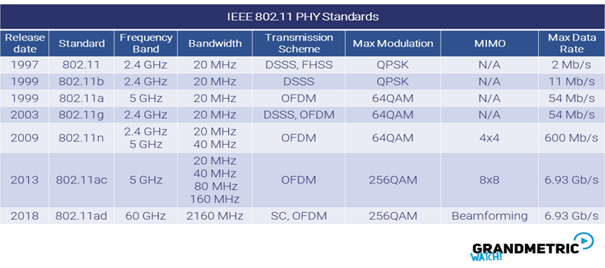
\includegraphics{obrazky/wifi-standards.png}
	\caption{Některé důležité verze standardu IEEE 802.11 a jejich parametry. Převzato z \url{https://www.grandmetric.com/2018/05/29/wi-fi-standards-evolution/}}
	\label{wifi-standards}
\end{figure}
Wifi funguje na principu vysílání a přijímání rádiových vln. Organizace IEEE rozhodla využít pro technologii Wi-Fi frekvence z pásma ISM [B, str.2]. Wifi standardně využívá frekvencí 2,4Ghz a 5Ghz. Nejprve byla zařízení Wi-Fi schopná pracovat pouze v jednom z těchto dvou frekvenčních pásem, ale 4. generace (IEEE 802.11n) přidává možnost práce v obou zmíněných pásmech. Moderní zařízení s wifi si tak mohou vybrat (a dokonce během své činnosti měnit) frekvenci, na které budou spolu komunikovat.
Obě pásma mají svá pro i proti. Mezi výhody pásma 2.4Ghz patří zejména větší pokrytí signálu a rovněž větší kompatibilita (platí spíše pro starší zařízení). Na druhou stranu pásmo 5Ghz nabízí podstatně vyšší přenosové rychlosti a dále větší množství komunikačních kanálů [D].

\subsection*{Režim sítě}
Wifi nachází uplatnění v (bezdrátových) lokálních sítích. V nich pak rozlišujeme 3 režimy na základě toho, jak se Wifi zařízení v síti mezi sebou navzájem spojují (jakou plní roli):
\begin{itemize}
    \item Režim infrastruktury
    \item Ad hoc režim
    \item Smíšený režim
\end{itemize}
V režimu infrastruktury je v sítí přítomen minimálně jeden centrální prvek (tzv. přístupový bod), který zprostředkovává komunikaci mezi jednotlivými prvky (klienty) sítě, případně poskytuje připojení do jiné sítě přes distribuční systém (DS). V tomto režimu sítě je výhoda, že je snadné připojit do stávající infrastruktury nový prvek. \newline
Ad hoc je režim bezdrátové sítě, ve které není přítomen žádný centrální prvek (přístupový bod) se kterým by prvky sítě komunikovali, ani zde není žádné spojení se pevnou sítí přes distribuční systém. Jedná se tedy o decentralizovanou síť. Jednotlivé prvky tedy mezi sebou navzájem komunikují přímo (toto spojení se někdy označuje jako tzv. peer-to-peer). V tomto režimu má síť rovněž SSID identifikátor, kterým je možné síť identifikovat. [A][B] \newline

\subsection*{Bezpečnost v síti Wi-Fi}
\todo{Todo...}
\section{Bezdrátový přenos pomocí Bluetooth}
Bluetooth je standard, definovaný v IEEE 802.15.1. Vytvořila jej firma Ericsson v roce 1994 a od té doby vyšlo několik nových verzí [A]. Podobně jako WiFi pracuje v ISM pásmu 2,4 GHz. Na rozdíl od Wi-Fi však není definován pouze na prvních dvou vrstvách ISO/OSI, ale definuje protokoly na všech sedmi vrstvách tohoto modelu. Na nejnižší úrovni, kde definuje způsob přenosu jednotlivých bitů využívá metodu FHSS, která zajišťuje, že při přenosu bitů vysílač přeskakuje mezi několika frekvencemi [AD].\newline
Zařízením, které jej využívají, umožňuje vytvořit tzv. PAN (osobní síť). V těchto sítích má každé zařízení přiřazeno unikátní 48bitovou adresu BD\_ADDR (BlueTooth Device Address) – jedná se o obdobu MAC adresy u ethernetu. Tu používá pro komunikaci s ostatními zařízeními. Jedno zařízení může být v roli master (řídící), slave (podřízená) nebo obojího [AB, str.4]. K jedné řídící stanici se připojuje jedno a více podřízených zařízení (používá se pouze adhoc komunikace mezi master a slave stanicí). Zde hovoříme o tzv. piconetu (pikosíti). Maximální počet zařízení v jedné pikosíti je 8 (jedna řídící stanice a až 7 podřízených). Stanice náležící do jedné pikosítě může zároveň patřit do jiné pikosítě. Jedná se tedy o rozšíření sítě mezi zařízeními. Takto vytvořenou síť nazýváme tzv. scatternet (rozprostřená síť). V každé rozprostřené síti má každá pikosíť unikátní identifikátor – je jím BD\_ADDR její řídící stanice. Díky rozlišení jednotlivých pikosítí pak může každá tato síť využívat jiné skokové sekvence (frekvenčních kanálů na kterých se vysílají/přijímají data) [AC, str. 20].

\section{Technologie ZigBee}
Zigbee je bezdrátová technologie, založená na standardu IEEE 802.15.4. Je určená pro vytváření sítě PAN (osobní síť) a pracuje v pásmu ISM 868 MHz, 902-928 MHz a 2,4 GHz [A]. 

\subsection*{Zařízení v ZigBee síti}
ZigBee standard specifikuje 2 typy zařízení – FFL (Full Function Device) a RFD (Reduced Function Device). FFL zařízení je obvykle schopné mnoha funkcí a je stále aktivní, zatímco RFD se nachází většinu času v režimu spánku, ze kterého se občas probudí, například aby odeslalo hodnoty neměřené na nějakém senzoru.\newline
V síti pak každé ze zařízení plní některou ze 3 funkcí:

\begin{itemize}
    \item Koordinátor
    \item Koncové zařízení
    \item Směrovač
\end{itemize}

\subsection*{Topologie sítě}
Na základě definovaných zařízení pak existují 3 možné topologie ZigBee sítě:

\begin{itemize}
    \item Hvězda
    \item Strom
    \item Mesh síť [AG, str.5]
\end{itemize}

\subsection*{ZigBee Model}
ZigBee podobně jako Bluetooth definuje komunikaci na všech úrovních modelu ISO/OSI, nekopíruje však přesně jednotlivé vrstvy. První 3 vrstvy modelů ISO/OSI a ZigBee si odpovídají, ale vrstvy L4-L7 jsou spojené do vrstev APS (Application Support) a ZDO (ZigBee Device Object). [AH, str. 42]\newline

Thread, WeMo, ZigBee and Z-Wave (https://www.tomsguide.com/us/smart-home-wireless-network-primer,news-21085.html)

\chapter{Vestavné systémy a vývojové prostředky}
\label{vestavne-systemy}
Následující část je shrnutím současného stavu v oblasti vestavných systémů a Python knihoven pro vývoj GUI aplikací. Není encyklopedickým výkladem problematiky, ale souhrnem informací, které mají k práci bezprostřední vztah. Nejprve je zde úvod do vestavných systému, následně je pojednáno o platformě Raspberry Pi, modulech ESP8266 a ESP32 a nakonec o možnostech programování GUI pomocí Python knihoven.

\section{Vestavný systém}

Vestavný systém můžeme definovat jako software spolu s počítačem, zabudovaným do nějakého zařízení takovým způsobem, že jej uživatel nevidí jako počítač [E, str.3]. Tento počítač je většinou jednoúčelový, určený pro předem navržené použití. Tím se liší od univerzálních počítačů, které mohou poskytovat různé funkce a jejichž uplatnění se může měnit (například osobní počítač) [F, str. 3].

\todo{Definovat mikropočítač, jednodeskový počítač, mikrokontrolér, mikroprocesor... (možná kapitola něco jako základní pojmy u vestavných systémů??}
\todo{Zkusit něco vytvořit z nějakého takového souhrnu: https://www.guru99.com/embedded-systems-tutorial.html}
\todo{https://jayconsystems.com/blog/microprocessor-vs-microcontroller-vs-microcomputer}
\todo{Historie smazána, vrátit ji? (Ale upravit!)}


\subsection*{Architektura řídícího zařízení}

Při návrhu systému se využívá jedna ze dvou architektur:

\begin{itemize}
    \item Von Neumannova architektura
    \item Harvardská architektura
\end{itemize}

Hlavním rozdílem je způsob práce s pamětí. Ve Von Neumannově architektuře je paměť pro program i data spojená do jedné paměti, v Harvardské architektuře je pak rozdělena. \newline
Mikroprocesor (CPU) je programovatelné elektronické výpočetní zařízení, určené pro všestranné použití. Jedná se o čip, obsahující 3 základní součásti:
\begin{itemize}
    \item Aritmeticko-logickou jednotku
    \item Řídící jednotku
    \item Registry [I, str. 18–19]
\end{itemize}

Mikroprocesor sám o sobě je z hlediska vestavěných systémů relativně jednoduché zařízení, které pro funkci systému potřebuje připojit některé další součásti, jako jsou paměti (RAM a ROM), čítače, časovač a podobně. Návrhář tedy musí tyto součásti přidat externě, aby zařízení fungovalo správně. Systémy, zahrnující mikroprocesory jsou obvykle založeny na Von Neumannově architektuře [J].\newline
Mikrokontrolér je zařízení, které na rozdíl od mikroprocesoru má již všechny součásti, potřebné pro svoji činnost v sobě. Obvykle využívá Harvardské architektury [J]. 

\section{Jednodeskový počítač Raspberry Pi}
Zařízení Raspberry Pi je levný univerzální počítač malých rozměrů. Poskytuje široké možnosti v oblasti multimédií a 3D grafiky, předpokládá se, že bude časem využíván i jako herní platforma.\newline
Název Raspberry Pi vytvořila komise dozorčí rady. Slovo Raspberry je vzato jako název ovoce (malina), jak už je u počítačových systémů zvykem nazývat podle ovoce. Slovo “Pi” označuje zkráceně “Python” - programovací jazyk, který měl být původně jediným programovacím jazykem dostupným na platformě Raspberry Pi [AA].

\subsection*{Historie}
Raspberry Pi vzniklo v r. 2006 za přispění studijního ředitele pro informatiku na Cambridgeské univerzitě za účelem lokálních potřeb. Měl to být nástroj, který by poskytl prvotní impuls studentů k nějakému z univerzitních kurzů.

\section{Moduly ESP8266 a ESP32}
Jedná se o levný mikročip, disponující Wi-Fi stackem, schopný provozu RTOS (realtime operačního systému). Je založen na 32bitovém procesoru s architekturou RISC [AE]. \newline
ESP32 je nástupce ESP8266. Kromě komunikace přes Wi-Fi umožňuje rovněž komunikaci pomocí Bluetooth, díky hybridnímu Wi-Fi/Bluetooth čipu [AF]. 


\begin{figure}[hbt]
	\centering
	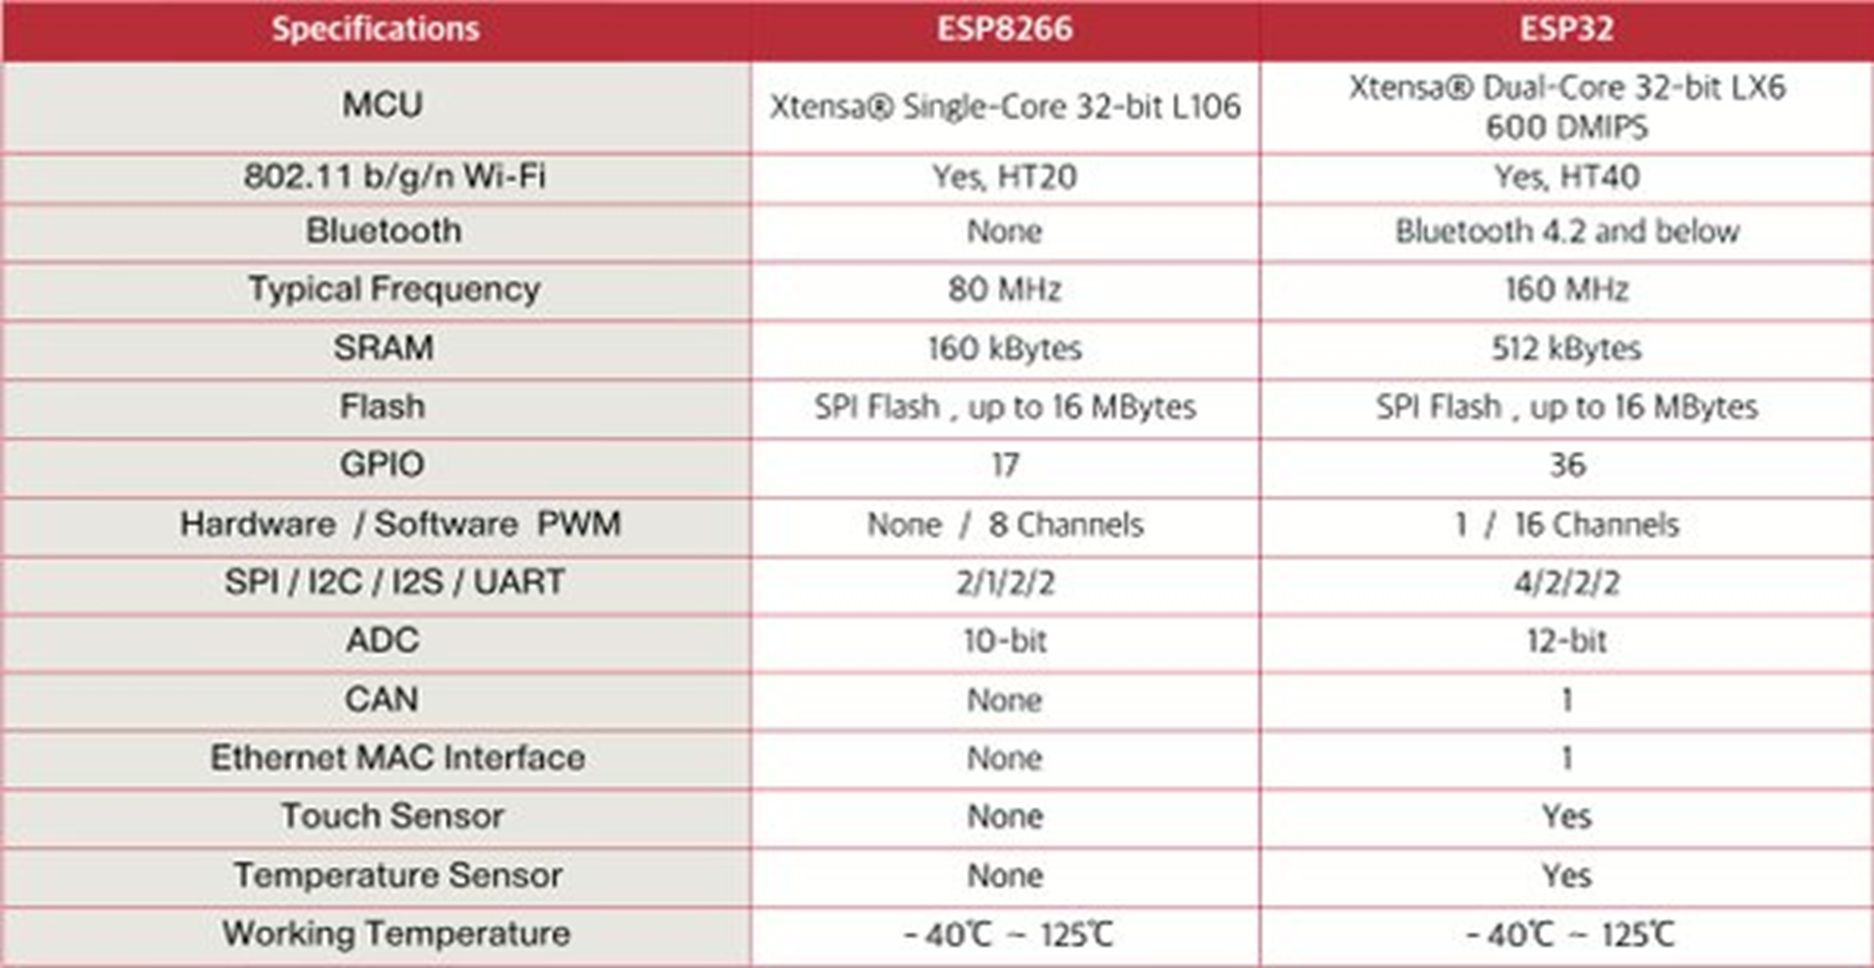
\includegraphics{obrazky/ESP.png}
	\caption{Srovnání specifikace modulů ESP8266 a ESP32. Převzato z \url{https://www.cnx-software.com/2016/03/25/esp8266-and-esp32-differences-in-one-single-table/}}
	\label{wifi-standards}
\end{figure}

\section{Python knihovny pro vývoj GUI}
K programování grafického uživatelského rozhraní existuje mnoho různých knihoven. Pro jazyk Python se nejčastěji používá některá z následujících knihoven:

\subsection*{Tkinter}

Knihovna tkinter je základní knihovna pro tvorbu okenních aplikací. Na rozdíl od ostatních knihoven je již obsažená v samotném jazyce Python, nemusí se tedy dodatečně instalovat [AL]. Používaní knihovny je tedy zdarma.\newline
Doporučuje se zvláště začátečníkům pro svou jednoduchost. Pro plnohodnotné využití je možné ke knihovně stáhnout dodatečné moduly [AM].

\subsection*{Kivy}

Knihovna Kivy patří mezi multiplatformní knihovny. Dle oficiálních stránek knihovny je možné vytvářet aplikace běžící na následujících zařízeních:

\begin{itemize}
    \item Desktopové počítače: OS X, Linux a Windows
    \item IOS zařízení: IPad a IPhone
    \item Android zařízení: tablety a telefony
    \item Jakékoli jiné dotykové zařízení, podporující TUIO (Tangible User Interface Objects) [AJ]
\end{itemize}

Knihovna přináší mnoho různých aspektů, které dle autorů knihovny mají zjednodušit tvorbu grafického rozhraní, obsluhu událostí a podobně.\newline
Ke knihovně rovněž patří zvláštní jazyk (nazvaný stejným jménem jako knihovna – jazyk Kivy). Jedním z jeho cílů je oddělení zodpovědnosti za prezentaci (zobrazení) a logiku programu [AK]. Zobrazení je dáno právě souborem kv (napsaném v jazyce Kivy) a logika souborem s Python kódem.\newline
Podobně jako tkinter, je i tato knihovna nabízena zdarma. Musí se však na rozdíl od tkinteru instalovat dodatečně.

\chapter{Zhodnocení současného stavu a plán práce}
V této kapitole se věnuji zhodnocení již existujících řešení automatizace domácnosti. Následně uvádím můj návrh řešení na základě nastudovaných řešení a vhodného rozsahu práce. Nakonec v bodech stanovuji cíle vyplývající z návrhu řešení, které se v práci snažím splnit.
\section{Současný stav}

Na trhu se v současné době nachází velké množství systémů. Z těch, které jsem popsal v části o existujících řešení je nejrozvinutějším systémem ten od společnosti Loxone. Zabírá opravdu širokou škálu možností a jen stěží by se hledala aplikace, pro kterou by nebyl vhodný. Kromě komplexnosti u něj oceňuji rovněž českou jazykovou lokalizaci. V češtině je k dispozici jak aplikace na ovládání (Loxone App), tak rovněž program pro konfiguraci systému (Loxone Config). Čím mě Loxone mile překvapilo je, že jsem si jejich aplikaci Loxone App mohl vyzkoušet v demoverzi i bez zakoupených komponent.\newline
Jako nevýhodu Loxone vidím příliš vysokou cenu. Uživatel, který si chce nainstalovat pár chytrých zařízení bude zřejmě překvapen cenou. Například při pořízení 3 chytrých zásuvek a miniserveru (který je k ovládání zásuvek potřebný) zaplatí přibližně 15 000 kč. Přitom adekvátní řešení od jiných firem, jako sonoff bude stát necelé 3000 kč, což je velký rozdíl – a při rozšiřování domácnosti o další prvky tento rozdíl znatelně roste. Na druhou stranu, pokud uživatel staví nový dům, může řešení od Loxone stát srovnatelnou cenu, jako konkurenční „neinteligentní“ instalace. Jako další nevýhodu vidím to, že celkově je instalace systému orientovaná spíše pro profesionální montáž pro pracovníky s příslušnou klasifikací (většina produktů je určena k zabudování do rozvaděče, příp. ke komunikaci s moduly v něm). Celkově je však řešení od Loxone na hodně vysoké úrovni.\newline

Řešení od firmy Jablotron je jistě zajímavé jejich dvoutlačítkovými (rozšiřitelnými) segmenty. Zdá se mi však nepraktické spojovat přístupovou klávesnici do domu s prvky automatizace domácnosti. Působí to poněkud omezeně. Navíc rozhraní pro ovládání domácnosti a alarmu v aplikaci MyJablotron se snaží napodobovat onu klávesnici, což příliš k přehlednosti nepřispívá. Na druhou stranu pro uživatele, jehož hlavní požadavek je zabezpečení objektu a pouze doplňková automatizace domácnosti (jako rozsvícení světel při odjištění domu) budou systémy od firmy Jablotron ideální.  \newline

Systém HomeKit je zajímavý v tom, že zde není potřeba žádný „speciální“ centrální prvek – pokud již uživatel vlastní například iPhone (či jiný produkt, který zastoupí funkci centrálního prvku). Nevýhodou je to, že aby byl systém ovladatelný globálně, tak je potřeba přeci jen mít v domácnosti nějaký prvek, co bude domácnost řídit. A pokud uživatel již nějaký nevlastní, tak se stává další investicí. Co je na systému HomeKit pozitivní je jeho nízká cena – ve srovnání se systémy od společnosti Loxone či Jablotron. Systém HomeKit se stále rozrůstá a má velkou podporu v rozmanitosti produktů. A na rozdíl od předchozích zmíněných systémů je více orientovaný na běžné uživatele. Jednou z nevýhod je zde to, že je systém orientovaný zejména na bezdrátovou komunikace, která samozřejmě někdy může být méně spolehlivá. Tím spíše že mnoho produktů komunikuje pouze pomocí Bluetooth, takže si uživatelé musejí hlídat dosah zařízení.\newline

Systém HomeConnect vnáší do automatizace domácnosti zajímavý koncept. Zatímco některé systémy umožňuji automatizovat domácnosti například chytrými zásuvkami či spínači, HomeConnect ve spolupráci s jinými společnostmi vyvíjí přímo spotřebiče s prvky chytré domácnosti, čímž tyto spotřebiče obsahují mnohem více „inteligence“, na rozdíl od pouhého „zapínání/vypínání“. Nicméně nevýhodou je zde příliš malý sortiment produktů, a tudíž jednoúčelová aplikace navíc, kterou stejně musejí uživatelé doplnit o další aplikace, chtějí-li například rovněž ovládat zásuvky, světla či rolety. Kromě toho je rovněž cena produktů dost vysoká.\newline
...

\section{Návrh řešení}
Na základě výzkumu dostupných řešení a jejich zhodnocení jsem se rozhodl vyvinout systém, který bude mít některé spíše základní funkce automatizace. Především zde bude řešeno dálkové ovládání jednoho zařízení druhým, jelikož je to zadání mé bakalářské práce. V systému tedy bude figurovat nějaký ovladač a dále ovládané prvky. 

V práci tudíž bude nutné zvolit vhodné vestavné zařízení, které bude sloužit jako ovládací část systému a také zařízení, která budou přijímat povely. Rozhodl jsem se, že ovládaný prvek zde nebude žádné konkrétní zařízení (jako zásuvka, spínač, či lampička) ale spíše nějaký obecný modul se vstupně výstupními porty, přes které bude možné ovládat jiná, už konkrétnější zařízení. Pro plnohodnotnou funkci systému bude tento modul nutné opatřit dalšími přídavnými součástkami. Půjde zejména o relé pro možnost ovládání zapnutí a vypnutí zařízení připojeného k tomuto modulu (tímto způsobem bude možné například ovládat LED pásek, či vytvořit bezdrátovou zásuvku). K modulu budou připojeny rovněž tranzistory pro možnost použití PWM modulace na výstupu - takový výstup pak bude sloužit pro stmívání světel, zejména LED pásku či bodových LED světel na 12 V. Ovládat tak bude možné rovněž servo motory, které se řídí PWM signálem.

Aby bylo ovládání systému co nejjednodušší, bude zde možnost ovládání na dotykovém displeji. Jelikož systém ovládaný jen z jednoho místa není v oblasti automatizace úplně nejšťastnějším a efektivním řešením (například uživatel sice nemusí dojít k vypínači světla, aby shasnul, ale stejně musí dojít někam k ovládacímu zařízení systému), rozhodl jsem se, že bude možnost ovládání i z telefonu, počítače a dalších zařízení (požadavky na zařízení budou definovaná později v části 6.X Návrh systému) \todo{Zmínit v implementaci požadavky}. Aby byl plněji využit potenciál displejů (ať už připojeného k ovládacímu zařízení, či ostatním zařízením, ze kterých bude možné moduly ovládat), rozhodl jsem se, že v systému bude možnost využívat několika různých senzorů.

Půjde o tyto senzory:
\begin{itemize}
    \item teploty
    \item pohybu
    \item sepnutí (kontaktu/tlačítka)
\end{itemize}
\todo{Uvést že dále budu ovládacímu zařízení říkat centrální prvek? Hub??}
Jde o typické představitele analogových i digitálních senzorů. Pro účely práce budou použity jen tyto tři, nicméně řešení chci pojmout jako open source (a s ohledem na tento fakt se budu snažit o co největší rozšiřitelnost systému), a další senzory bude možné přidat v budoucnu. Všechny senzory budou mít v systému pouze informativní charakter pro uživatele, tzn. bude si moci například zobrazit teplotu v konkrétní místnosti, zda se v ní někdo nachází, či zda byl sepnut nějaký kontakt (např. dveře). Nebude možné přímo systém pomocí senzorů ovládat, ale opět nic nebrání tomu, aby byla tato funkce implementována v budoucnu. U modulů s výhodou využiji, že budou mít více vstupů/výstupů a jeden modul tak může sdružovat více různých funkcí (například mít připojené 2 různé senzory a ovládat 5 výstupů).

Mým řešením bych chtěl doplnit existující open source řešení o takové, které bude svými vlastnostmi určeno spíše pro kutily v oblasti automatizace domácnosti. Bude poskytovat jednoduchý systém pro ovládání mnoha zařízení pomocí jednoho vestavného zařízení s připojeným displejem. Svou prací bych si chtěl rovněž vyzkoušet celý návrh a realizaci systému automatizace domácnosti, který bych následně mohl sám využívat. Vylepšením oproti některým již existujícím systémům bude možnost sdružení několika přijímajících zařízení do jednoho (jak jsem zmínil v předchozím odstavci).

Při práci budu využívat již existující moduly a mikropočítač (který bude sloužit jako „mozek“ systému), které však naprogramuji a vhodným způsobem doplním o některé elektronické součástky (jako zmíněné relé, či tranzistor). Práce se však nebude zabývat konstrukčním návrhem prvků systému, ani návrhem DPS pro hotový systém. Pro případně spojení komponent systému budou použita nepájivá kontaktní pole.

\section{Cíle práce}
Na základě předchozích úvah jsem se rozhodl, že vytvořím systém, který bude splňovat následující vlastnosti:

\begin{itemize}
    \item Bude zvolen vhodný mikropočítač, který bude sloužit jako ovládací část systému
    \item Pro ovládací část bude zvolen dotykový displej patřičných rozměrů, aby byl systém přehledný a mohl sloužit pro ovládání zařízení
    \item Displej by měl být rovněž vybrát s ohledem na možnost zobrazení přehledu o stavu zařízení v systému (například. zobrazení, které zařízení jsou zapnutá, či jaké hodnoty se nacházejí na PWM výstupu)
    \item K implementaci bude zvolen vhodný programovací jazyk
    \item Bude podporována funkce přímého ovládání výstupů ovládaných modulů
    \item Také zde bude funkce zobrazení dat ze senzorů
    \item Systém bude obsahovat českou jazykovou lokalizaci
    \item K systému bude možné přistupovat jak lokálně, tak i vzdáleně
    \item Pro vzdálený přístup zde budou fungovat uživatelské účty, přičemž z jednoho účtu bude možné ovládat jen jednu domácnost
    \item Bude zvolena vhodná technologie bezdrátového přenosu tak, aby byl systém co nejjednodušší na implementaci a případné rozšiřování
    \item Projekt bude uvolněn jako open source, čímž bude cena systému jako takového pro potenciální uživatele minimální (daná pouze cenou použitých součástek a zařízení)
\end{itemize}

\chapter{Realizace a testování}
V této kapitole se věnuji vlastní realizaci řešení a následnému testování a vyhodnocení. V první podkapitole uvádím celkový návrh systému -tedy z jakých aplikací a zařízení se bude skládat, jak mezi sebou budou komunikovat apod. Následně se věnuji návrhu grafického uživatelského rozhraní pro aplikaci, ke kterým uživatel bude přistupovat. V dalších kapitolách již rozebírám implementaci konkrétních aplikací. Nakonec uvádím jak jsem systém testoval a k jakým výsledkům testy vedly.
\todo{Někde vymezit pojmy...klient, klientská aplikace, (koncový) modul...}
\section{Celkový návrh systému}
Systém se bude skládat celkem ze tří aplikací a několika zařízení (každé zde bude mít svou roli). 

\subsection*{Zařízení}
Jmenovitě budou v systému fungovat tato zařízení:
\begin{itemize}
    \item Centrální jednotka (s připojeným displejem)
    \item Koncové moduly
    \item Senzory
    \item Ovládaná zařízení
    \item Ostatní zařízení, přes která bude možné systém ovládat (klienti)
\end{itemize}

Centrální jednotka bude mít na starosti celý systém řídit. Pokud například uživatel zadá pokyn ke změně hodnoty na některém výstupu modulu, bude to právě Centrální jednotka, kdo tuto žádost (v jistém smyslu) přijme a pošle ji dále jako příkaz na konkrétní koncový modul.
Jelikož k centrální jednotce bude potřeba připojit (dotykový) displej, musí mít dostatečný výkon pro vykreslování na něj a zpracování dat. Bylo tedy potřeba zvolit vhodný mikropočítač (protože mikrokontrolery mívají obecně daleko menší výkon) opatřený nějakým portem pro přenos obrazu. Jedním z nejpoužívanějším a také nejrychleji vyvíjejícím se mikropočítačem je Raspberry Pi, vlastní ho tedy již mnoho IT\todo{?} nadšenců. Je relativně levné (ve verzi 3 se dá sehnat do jednoho tisíce kč, verzi Zero W je dokonce možné na českém trhu sehnat za přibližně 300 kč) a tedy i snadno dostupné. Nadto je použití Raspberry Pi doporučeno v zadání mé práce.

Koncový modul (dále již jen modul) bude zařízení, které bude mít nějaké vstupy a výstupy. Modul bude měnit hodnoty na svých výstupech dle instrukcí, přicházejících z centrální jednotky. K těmto výstupů pak budou dále připojeny příslušné součástky (jako relé, či tranzistor) a k nim dále již reálná zařízení, ve kterých budou nějakým způsobem spínat kontakt. Rovněž bude v pravidelných intervalech číst hodnoty na svých vstupech (ke kterým budou připojeny senzory). Jako koncový modul je potřeba vybrat zařízení s nízkou cenou, jelikož těchto zařízení může být i více. Kromě toho bude modul přijímat pouze jednoduché příkazy od Raspberry Pi, může se tedy klidně jednat o nějaký mikrokontroler s omezeným výpočetním výkonem. Je však potřeba, aby byl tento mikrokontroler schopný komunikovat po síti (tento požadavek vyplývá ze zadání mé bakalářské práce). Na trhu existují především 2 takové mikrokontrolery - ESP8266 a novější ESP32.

Ovládanými zařízeními zde myslím ta, co budou připojena na některý z výstupů modulu. Půjde tedy například o LED pásek, či zařízení, u kterého bude spínat kontakt.

Klientská zařízení budou libovolná zařízení, přes které bude uživatel moci ovládat systém. Jedinými požadavky na tato zařízení jsou zde vzhledem k implementaci:
\begin{itemize}
    \item Přístup k internetu
    \item Dostatečně velký displej (ideálně 5´´ a více)
\end{itemize}

\subsection*{Aplikace}
Dále kromě zařízení budou v systému fungovat tyto tři aplikace:
\begin{itemize}
    \item Klientská aplikace (dále již jen klient), určená jako grafické rozhraní pro uživatele k ovládání systému
    \item Server, který bude od klienta (ať už přímo, nebo zprostředkovaně skrze databázi) získávat instrukce a vykonávat je
    \item Aplikace na modulech
\end{itemize}

Po úvaze jsem dospěl k názoru, že nejvhodnější bude, když bude klient implementován jako jednostránková webová aplikace. A to z několika důvodů:
\begin{itemize}
    \item Webové aplikace jsou obecně vzato multiplatformní (pokud mají alespoň trochu responzivní design), čehož vhodně využiji v rámci možnosti ovládat domácnost i na dálku
    \item K přístupu k aplikaci tak bude stačit mít zařízení s přístupem k internetu (a obrazovkou pochopitelně)
    \item Webové technologie patří mezi rychle se rozvíjející, což přispívá k budoucímu rozvoji systému
    \item Jazyk Typescript (který budu používat) je jeden z vůbec nejpoužívanějších a nejznámějších programovacích jazyků, pokud se tedy najde programátor, který by chtěl v budoucnu systém rozšířit, je velká pravděpodobnost se nebude muset učit nic nového.
\end{itemize}

\begin{figure}[!hbt]
	\centering
	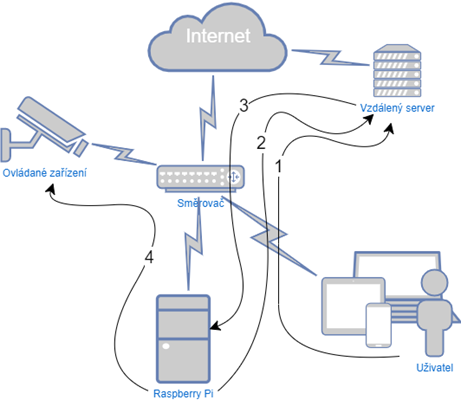
\includegraphics[scale=0.7]{obrazky/architektura.png}
	\caption{Architektura systému pro automatizaci domácnosti}
	\label{architektura}
\end{figure}
\todo{Upravit scale obrázku výše!}

Druhá aplikace pak bude běžet na Raspberry Pi jako server zpracující požadavky jednak od klientů, a pak také samozřejmě požadavky zadané přímo na displeji Raspberry Pi \todo{...rozvést...}


Jako alternativu těchto prvních dvou aplikací bylo možné vytvořit jen jednu, běžící na Raspberry Pi, přes kterou by se systém ovládal pouze z připojeného displeje. Nicméně tímto by se ztratila možnost ovládat systém i vzdáleně, resp. i z jiných zařízení, než je Raspberry Pi, což by bylo jistě neintuitivní a mnohdy nepříjemné, zvolil jsem tedy řešení dvou aplikací.

\subsection*{Programové prostředky}
\todo{Vysvětlit proč jsem si vybral zrovna typescript a node.js a jaké jsou alternativy (a alternativní řešení)}

\subsection*{Celková architektura systému}
\todo{Uvést celkově co s čím a jak bude komunikovat, dle obrázku \ref{architektura} (a vytvořit nový)}

Na obrázku \ref{architektura} je možné vidět celkovou koncepci systému.


\section{Grafický návrh klientské aplikace}
Aplikace byla rozdělena na několik samostatných částí (oken), mezi kterými může uživatel přecházet. Jelikož se jedná o jedno stránkovou aplikaci, nejde v případě jednotlivých částí o klasické stránky (v tom smyslu, že by každá měla vlastní html dokument, který ji generuje). V následujícím textu se však budu odkazovat ke každému takovému samostatnému oknu, jako k jedné (webové) stránce.
\subsection*{Přihlašovací stránka a registrace}
Na úvod při spuštění se zobrazí stránka, na které se uživatel bude moci přihlásit (pomocí emailu a hesla). Rovněž zde bude možnost přejít k registraci nového účtu, vyžádat si zapomenuté heslo či projít dále do aplikace bez přihlášení (tato možnost bude pouze v aplikaci Raspberry Pi).

\subsection*{Menu}
V aplikaci se přihlášenému uživateli bude zobrazovat vyjíždějící menu, kterým se bude moci přepínat mezi jednotlivými stránkami (jako domovská stránka či nastavení). V menu také bude možnost odhlášení, která však pravděpodobně nebude často využívána.
\subsection*{Domovská stránka}
Za domovskou stránku považuji tu, na kterou se uživatel dostane ihned po přihlášení do systému. Tato stránka bude sloužit i jako výchozí pro ovládání jednotlivých zařízení. Bude zde také přehled hodnot na senzorech. Tuto stránku bude mít uživatel zobrazenou většinu času na displeji Raspberry Pi, pokud jej bude chtít používat jako takový rychlý přehled o stavech ovládaných zařízení (a senzorech).
Jak vidíme na obrázku XYm bude tato stránka rozvržena na jednotlivé místnosti. Pro každou zde bude pod sebou vyhrazené místo a v něm pro každou místnost se stejným rozvržením - název místnosti, seznam hodnot na senzorech a ovládaná zařízení (ze kterých bude možné vyčíst jejich stav i ovládat je). Pokud bude chtít uživatel ovládat nějaké zařízení, klikne na něj. V případě zařízení typu zapnuto/vypnuto se okamžitě změní stav zařízení. V případě zařízení, řízených PWM modulací se zobrazí nad zařízeními posuvník (nastavený na aktuální hodnotu), kterým bude možné okamžitě měnit hodnotu na výstupu modulu (a tedy stav zařízení).

\subsection*{Nastavení}
V aplikaci bude také stránka s nastavením. Bude zde možnost přidávat nová zařízení a konfigurovat ta stávající...
\todo{Dodělat...Nebude zde nastavení a konfigurace zvlášť?}


\section{Implementace klientské aplikace}
\todo{Zmínit že spárování uživ. účtu s RPi bude tím, že se přihlásí uživatel na lokálním serveru}
\section{Implementace serveru na Raspberri Pi}
\section{Implementace aplikace pro koncové moduly}
\section{Testování a vyhodnocení systému}


\subsection*{Provedené testy}
V rámci testování jsem provedl tyto testy:
\begin{itemize}
    \item Test reaktivity
    \item Test intuitivnosti uživatelského prostředí
    \item Test stability při potížemi s připojením k internetu
    \item Test autonomie?
\end{itemize}

Test reaktivity (neboli odezvy systému na podněty v reálném čase) probíhal takto...

Test intuitivnosti uživatelského prostředí probíhal takto...

Test Test stability při potížemi s připojením k internetu probíhal takto...

Test autonomie (funkce systému bez lidského zásahu) probíhal takto...

\subsection*{Testy které nebyli provedeny}
Kromě testů, které jsem už provedl by bylo vhodné provést ještě dále zmíněné. V případě absence prvních dvou nedojde k žádným potížím (jen systém možná nebude fungovat na jiných zařízeních). Problémy, které by se otestovali zbylými dvěma testy by však mohli být kritické. Alespoň u čtvrtého testu ale věřím, že nejsou obavy na místě, přeci jen je konkurence velká a systém by neměl být zahlcený. V rámci mé práce tyto testy vykonány nebyli, zejména z finančních a časových důvodů.
Testy které by bylo vhodné provést:
\begin{itemize}
    \item Funkčnost systému na alternativních mikropočítačích 
    \item Funkčnost systému na jiných verzích Raspberry Pi
    \item Stabilita systému v průběhu několika let chodu
    \item Test spolehlivosti systému při velkém množství uživatelů
\end{itemize}
Raspberry Pi je jedním z nejpoužívanějších a nejznámějších mikroprocesorů, nicméně na trhu se nacházejí další, u kterých by bylo vhodné otestovat, zda bude server i klientská aplikace (na připojeném displeji) plně funkční. Zejména mikropočítače uvedené v kapitole \ref{vestavne-systemy} (tam jsem totiž popisoval rovněž nejpopulárnější mikropočítače)

Funkčnost systému na jiných verzích Raspberry Pi je potřeba otestovat zejména z toho důvodu, že se jedná o poměrně rychle se rozvíjející platformu a někteří potenciální uživatelé tak mohou mít starší model s nižším výkonem. Zvláště zajímavý by byl test na verzi Zero W, jelikož tuto verzi Raspberry Pi je možné pořídit za přibližně 300 kč. V případě bezproblémového chodu by byl projekt velmi zajímavou alternativou k některým velmi drahým systémům jako je \todo{XYZ}. Je možné, že by například nebyla tato verze Raspberry Pi dostatečně výkoná na ovládání systému z připojeného displeje, ale zvládala by na běh aplikace serveru, pak by bylo možné systém prostě ovládat z klientů (například chytrých telefonů). Případně kdyby tato verze nezvládala bezproblémový běh serveru s poskytováním statické stránky, tak by bylo možné tuto část serveru upravit (odstranit) a pak by se klienti připojovali pouze na vzdálený server a úloha Raspberry Pi by se zredukovala pouze na kontrolu (resp. naslouchání) změn v databázi a komunikaci s koncovými moduly, což by snad mělo opravdu bez jakýchkoli potíží fungovat. Pak by se samozřejmě muselo vyřešit spárování Raspberry Pi s uživatelským účtem, protože aktuálně to funguje právě na principu, který vyžaduje, aby se uživatel (alespoň poprvé) přihlásil na poskytované statické stránce z Raspberry Pi.

Test stability systému by pak spočíval v tom, že by systém pravidelně po dobu několika let využívalo jisté množství lidí (například 100 domácností) a pozorovalo, zda se systém v průběhu času chová stále stejně, nezpomaluje se a podobně.

Test spolehlivosti systému při velkém množství uživatelů by bylo provést hlavně z toho důvodu, že v systému funguje jedna veřejná databáze. Vylo by vhodné otestovat, jak se systém bude chovat při velké zátěži databáze (ve chvíli, kdy bude k databázi aktivně současně přistupovat mnoho uživatelů).






























\chapter{Závěr}
\label{zaver}

Nápady na pokračování práce:
\begin{itemize}
    \item ovládání hlasem
    \item přidání podmínek
    \item přidání módů (scén) - v podstatě by se jednalo o sdružení více akcí ovládání do jedné
    \item vývoj by mohl směřovat i na odlehčení serveru tak, že bude pouze kontrolovat databázi a komunikovat s moduly (jak bylo polemizováno v testování) => a mohla by se vytvořit verze pro ESP8266 v režimu Centrální jednotky => velice levný systém...
\end{itemize}

Moje odkazy \cite{4technologie} \cite{BezdratoveSite} \cite{DesigningEmbeddedSystems} \cite{EmbeddedSystems}
\cite{EmbeddedSystemsCircuits}
\cite{ITURegulations} \cite{MicroprocessorAndInterfaces} \cite{WifiFrequencyBands} \cite{uCvsCPU} \cite{arduino} \cite{ArduinoProgramming} \cite{whatIsIR} \cite{optics} \cite{physics} \cite{HomeAutomationRPI} \cite{Everything2_4GHZ} \cite{microwave} \cite{materials} \cite{wirelessComunication} \cite{NetworkSecurity} \cite{RPiPrirucka} \cite{BluetoothGuide} \cite{WirelessPersonalCommunications} \cite{GettingStartedBluetooth} \cite{Why2_4GHz} \cite{ESP8266} \cite{ESP32} \cite{HandsOnZigBee} \cite{ZigbeeWirelessNetworking}


%===============================================================================
